\section{Model}
\subsection{Gradient $k$-means}
Most implementations of $k$-means work without the use of gradient methods, usually by using Lloyd's algorithm 
\cite{lloyd}. However, a gradient descent version of $k$-means is fairly simple to derive. Following the derivation provided by Bottou and Bengio \cite{convergence}, we frame $k$-means as the following minimization problem:
\begin{equation}
\min \mathcal{L} = \min \sum_{i=1}^N \frac{1}{2} ||x_i - c_{x_i}||^2
\end{equation}
where $c_{x_i}$ is the closest cluster center to data point $x_i$. This then gives the following gradient: 
\begin{equation}
\frac{\partial \mathcal{L}}{\partial c_j} = \sum_{i=1}^N 
\begin{cases}
x_i - c_j  &  \text{if } c_j = c_{x_i} \\
0& \text{else} \\
\end{cases}
\end{equation} 
With the gradient in hand, we can use a gradient descent algorithm to perform $k$-means clustering. In fact, Sculley has shown that a mini-batched version of this approach converges faster than any other algorithm when working in a large data regime \cite{Sculley}. We will call this model gradient $k$-means. As a baseline for my model, I implemented mini-batched gradient $k$-means in Tensorflow, which did not exist elsewhere to the best of my knowledge. Table \ref{sklearn} shows that it generates clusterings of higher quality than the algorithm provided by scikit-learn.\footnote{\texttt{http://scikit-learn.org/stable/modules/generated/sklearn.cluster.MiniBatchKMeans.html}}

\begin{table}
	\caption{Comparison of $k$-means implementations. We compare scikit-learn's MiniBatchKMeans method$^2$  and my gradient $k$-means implementation. We see that my implementation results in higher quality clusterings for both datasets (Section 5.1).}
	\label{sklearn}
	\begin{center}
	\begin{tabular}{|c |c c |c c|}
		\multicolumn{1}{c}{} & \multicolumn{2}{c}{MNIST}   &\multicolumn{2}{c}{EMNIST}   \\
		\hline
		Score & scikit-learn & Gradient $k$-means & scikit-learn & Gradient $k$-means\\
		\hline \hline
	    V-Measure & 0.514 & 0.533 & 0.466 & 0.467 \\ 
		NMI & 0.387 & 0.441 & 0.368 & 0.372\\  
		Rand Score & 0.138 & 0.338 & 0.089 & 0.185\\
		\hline
	\end{tabular}
	\end{center}
\end{table}

\subsection{Autoencoded $k$-means}
Since gradient $k$-means produces gradients, we can backpropagate the error signal from the $k$-means objective through a neural architecture. I have a designed a  model which consists of an autoencoder whose hidden state is given as input to gradient $k$-means (Figure \ref{fig:grad_kmeans}). We will refer to this model as autoencoded $k$-means. During training, the error signals from both the autoencoder reconstruction and gradient $k$-means is backpropagated jointly through the hidden state. In this way, we are not only learning a smaller representation for the input, we are biasing that representation to be well suited for clustering. The objective for the entire architecture is: 
\begin{equation}
\frac{1}{N}\sum_{i=1}^N \frac{1}{F} ||x_i-x_i'||^2 + \frac{1}{N}\sum_{i=1}^N \frac{1}{2} ||h_i - c_{h_i}||^2
\end{equation}
where $F$ is the number of features.
\begin{figure}
	\begin{center}
		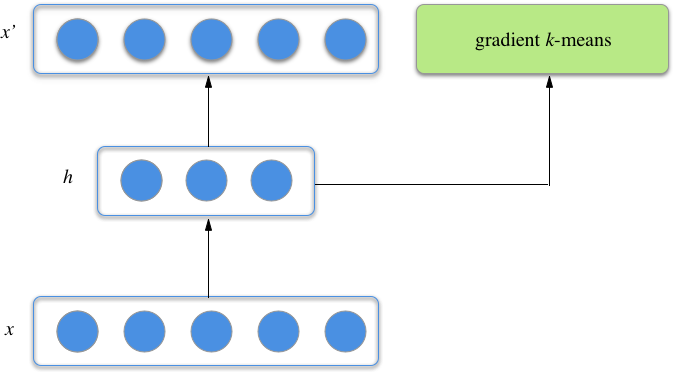
\includegraphics[width=0.6\textwidth]{figs/akm.png}
	\end{center}
	\caption{The autoencoded $k$-means architecture.}
	\label{fig:grad_kmeans}
\end{figure}